\documentclass{article}
\usepackage{graphicx} % Required for inserting images
\usepackage[utf8]{inputenc}
\usepackage[vietnamese]{babel}
\usepackage{indentfirst}
\usepackage{biblatex}
\usepackage{tikz}
\usetikzlibrary{calc}
\usepackage{listings}
\usepackage{courier}
\usepackage{soul}
\usepackage[utf8]{inputenc}
\usepackage[a4paper, margin=0.4in]{geometry}
\newcommand\HRule{\rule{\textwidth}{1pt}}
\usepackage[colorlinks=true, urlcolor=blue]{hyperref}
\usepackage{enumitem}
\usepackage{xcolor}

\begin{document}
\begin{titlepage}

\begin{center}

TRƯỜNG ĐẠI HỌC KHOA HỌC TỰ NHIÊN\\
\textbf{KHOA CÔNG NGHỆ THÔNG TIN}\\[2cm]

{ \large \bfseries Nguyễn Đức Tài - Phạm Hoàng Hải Đăng\\ Lê Hồng Thạch - Trần Đình Tấn Phát\\ Phan Nguyễn Gia Huy - Nguyễn Đỗ Bảo Kiên\\[2cm] } 


{ \large \bfseries \textbf{ĐỒ ÁN LÍ THUYẾT GIỚI THIỆU TRÍ TUỆ NHÂN TẠO} \\[3cm]} 


\large \textbf{ IMAGE CAPTIONING }\\

\large CHƯƠNG TRÌNH CHÍNH QUY\\

\begin{tikzpicture}[remember picture, overlay]
  \draw[line width = 2pt] ($(current page.north west) + (1cm,-1cm)$) rectangle ($(current page.south east) + (-2cm,1cm)$);
\end{tikzpicture}

\vfill
Tp. Hồ Chí Minh, tháng /2024

\end{center}

\pagebreak
\end{titlepage}
\maketitle

\tableofcontents

\textbf{ĐÁNH GIÁ THÀNH VIÊN}:
\begin{itemize}
    \item Nguyễn Đức Tài: nhiệt tình, chăm chỉ, hoạt bát. 
    \item Phạm Hoàng Hải Đăng: chăm chỉ, chịu khó,  .
    \item Lê Hồng Thạch: nhiệt tình, chịu khó.
    \item Trần Đình Tấn Phát: năng nổ, hoạt bát.
    \item Phan Nguyễn Gia Huy: cần cù, chăm chỉ.
    \item Nguyễn Đỗ Bảo Kiên: hòa đồng, chăm chỉ.
\end{itemize}

\textbf{ĐÁNH GIÁ MỨC ĐỘ HOÀN THÀNH CHO TỪNG YÊU CẦU}:
\begin{itemize}
    \item Source code: xong 
    \item slide: xong
    \item Report:xong
\end{itemize}

\maketitle

\section{Introduction: Giới thiệu bài toán.}
\subsection{Khái niệm: }
Image-captioning là việc làm cho máy tính có thể tự sinh mô tả cho một bức ảnh được nhập vào. Giống như cách mà chúng ta nhìn vào một bức ảnh và hiểu bức ảnh đó có nội dung là gì, máy tính cũng có thể làm tương tự.\\
VD:
\begin{figure}[h]
  \centering
  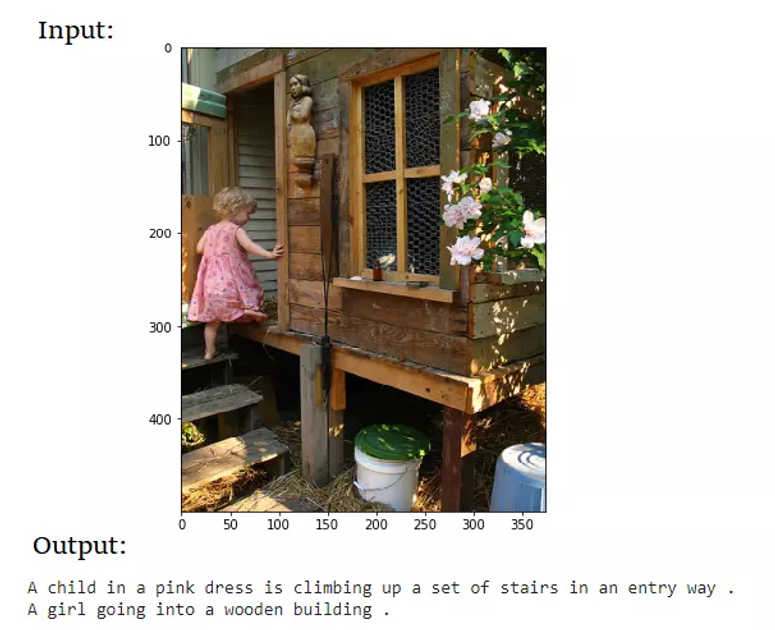
\includegraphics[width=0.9\textwidth]{img/anh1.png}
  \label{fig:my_label}
\end{figure}
\subsection{Ứng dụng của image-captioning:}
\renewcommand{\labelenumi}{\alph{enumi}.}
\begin{itemize}
    \item Sinh mô tả cho ảnh: Số lượng ảnh lớn, khổng lồ việc gán nhãn thủ công sẽ mất thời gian và tiêu tốn tiền bạc. Hãy để AI gãn nhãn dùm
    \item Các ứng dụng hỗ trợ người khiếm thính ( tích hợp với chuyển text thành audio để mô tả ảnh cho người bị mù…)
    \item ETC…
\end{itemize}
\subsection{Cách mà mô hình image captioning hoạt động:}
Hãy nghĩ về chú thích hình ảnh như một sự hợp tác giữa hai thành phần thiết yếu của bộ não máy tính:
\renewcommand{\labelenumi}{\alph{enumi}.}
\begin{itemize}
    \item Con mắt (Mạng thần kinh tích chập - CNN): Cũng giống như chúng ta có mắt để nhìn, máy tính có CNN để phân tích hình ảnh. Các mạng này giúp máy tính xác định các yếu tố quan trọng trong hình ảnh, chẳng hạn như tai hoặc đuôi của mèo. Những yếu tố chính này được dịch thành một tập hợp các số đặc biệt mà máy tính hiểu được. Những số đặc biệt này được gọi là "vector embeddings".
    \item Miệng (Mạng thần kinh tuần hoàn - RNN): "Miệng" của máy tính là RNN. Nó lấy những con số đặc biệt đó (vector embeddings) từ CNN và kết hợp chúng với sức mạnh của từ ngữ. Nó giống như thể chúng ta đang dạy máy tính thuật lại một câu chuyện về hình ảnh. RNN lấy từng từ một và bắt đầu tạo thành một câu. 
\end{itemize}
\section{Methodology: Giải thích phần xử lý dữ liệu, giới thiệu mô hình, giải thích mô hình.
Phần này t chỉ làm cái sườn chính thôi nên ae tự tìm kiếm them thông tin để soạn rõ hơn từng bước!
}
\subsection{Xử lý dữ liệu (Data Preprocessing)}
\subsubsection{Chuẩn bị dữ liệu chú thích ảnh (Captions):}
Dữ liệu thường được sử dụng có thể là bộ Flickr 8k, Flickr 30k hoặc bộ dữ liệu MS COCO. Ở đây mình sử dụng dữ liệu Flickr 8k được tải trực tiếp từ kaggle. Cách tải các bạn có thể xem trong file notebook.

Dữ liệu bao gồm một bộ 8000 ảnh và một file captions.txt. Mỗi ảnh sẽ có 5 captions làm nhãn. Cấu trúc file như sau:
\begin{figure}[h]
  \centering
  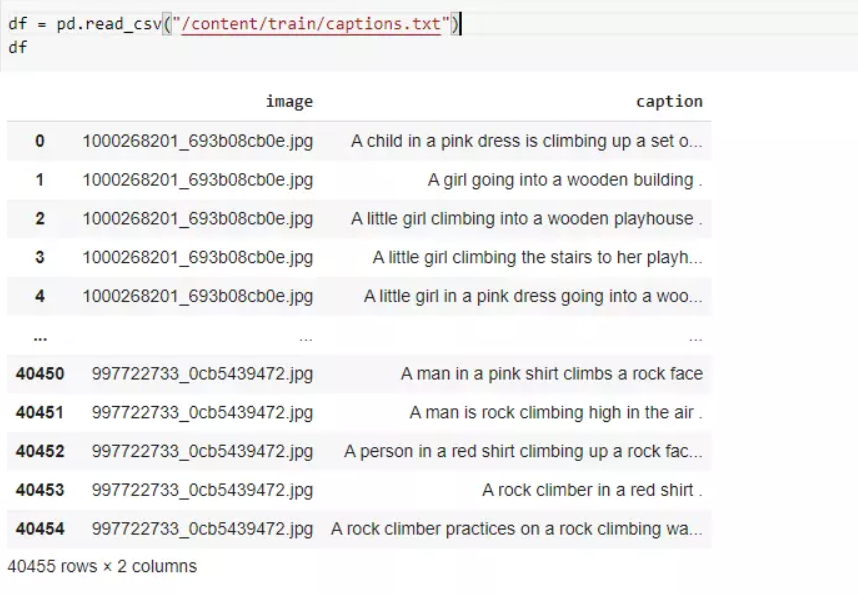
\includegraphics[width=0.75\textwidth]{img/anh2.png}
  \label{fig:my_label}
\end{figure}\\
Image size của data này là (500,375,3)\\

Ví dụ về 1 ảnh và 5 captions của nó:\\
\begin{verbatim}
        n = 17
        img = Image.open(image_path + df['image'][5*n])
        plt.figure(figsize=(7, 7))
        plt.imshow(img)
        print(df['caption'][5*n:5*n+5])
\end{verbatim}
\begin{figure}[h]
  \centering
  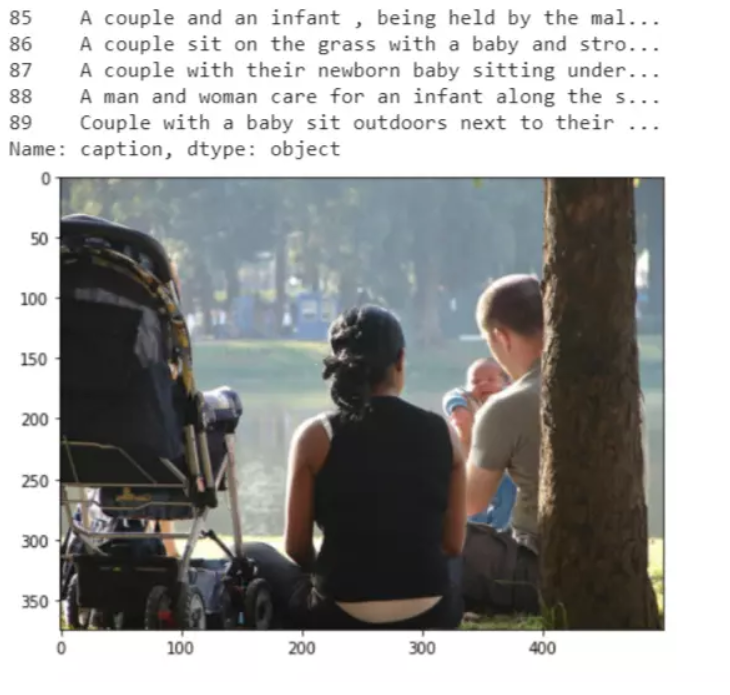
\includegraphics[width=0.75\textwidth]{img/anh3.png}
  \label{fig:my_label}
\end{figure}
\begin{itemize}
    \item Từ tệp captions.txt, các chú thích được tải lên và ánh xạ vào các hình ảnh tương ứng thông qua mã hình ảnh (image ID).
    \item Mỗi hình ảnh có 5 chú thích mô tả, tổng cộng có 40,455 chú thích cho 8,091 hình ảnh.
\end{itemize}
\subsubsection{Tiền xử lý chú thích:}
\begin{itemize}
    \item Chuyển toàn bộ văn bản sang chữ thường (lowercase).
    \item Loại bỏ các ký tự không phải chữ cái (non-alphabetical characters).
    \item Xóa các khoảng trắng thừa.
    \item Thêm các token đặc biệt startseq và endseq để đánh dấu điểm bắt đầu và kết thúc của mỗi chú thích.
\end{itemize}
Ví dụ:
\begin{figure}[h]
  \centering
  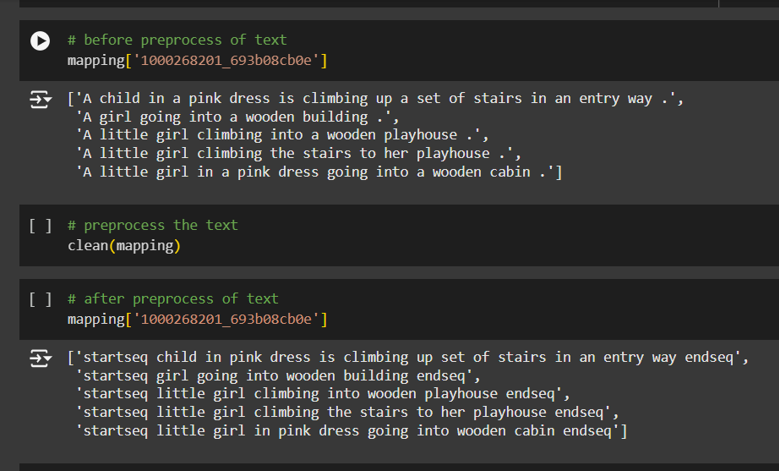
\includegraphics[width=0.75\textwidth]{img/anh4.png}
  \label{fig:my_label}
\end{figure}
\subsubsection{Token hóa văn bản (Tokenization):}
\begin{itemize}
    \item Sử dụng Tokenizer để chuyển đổi các từ trong chú thích thành các chỉ số số học, tạo điều kiện cho mô hình học tập.
    \item Lưu tokenizer vào tệp để tái sử dụng trong các bước sau.
\end{itemize}
\subsubsection{Kích thước từ vựng và độ dài tối đa:}
\begin{itemize}
    \item Kích thước từ vựng: 8,768 từ.
    \item Độ dài chú thích tối đa: 34 từ.
\end{itemize}
\subsection{Giới thiệu mô hình (Model Introduction)
Mô hình bao gồm hai thành phần chính:
}
\subsubsection{Trích xuất đặc trưng từ hình ảnh:}
\begin{itemize}
    \item Sử dụng mô hình VGG16 đã được huấn luyện trước trên tập dữ liệu ImageNet để trích xuất đặc trưng từ hình ảnh.
    \item Lớp Fully Connected (FC) cuối cùng của VGG16 bị loại bỏ để chỉ giữ lại các đặc trưng dạng không gian.
\end{itemize}

\section{}
\subsection{Xử lý ngôn ngữ tự nhiên (Natural Language Processing - NLP): }
 
Sử dụng mô hình LSTM (Long Short-Term Memory) để tạo ra các chú thích từ các đặc trưng hình ảnh.
\\
LSTM là một loại mạng nơ-ron hồi tiếp (RNN) giúp xử lý dữ liệu chuỗi (như văn bản) và có khả năng ghi nhớ thông tin dài hạn, rất phù hợp cho bài toán tạo chú thích ảnh.


\section{ Giải thích mô hình(Model Explanation)}
\subsection{ Kiến trúc mô hình}
\begin{itemize}

    \item \textbf{Đặc trưng hình ảnh(Image Feature)}
    \\
    Các đặc trưng từ VGG16 được nén lại thành một đầu vào vector.\\
\\
    VGG16: Một mạng nơ-ron CNN (Convolutional Neural Network) được sử dụng để nén hình ảnh thành một đầu vào vector. VGG16 đã được huấn luyện trên ImageNet và có thể chuyển đổi hình ảnh thành các đặc trưng mạnh mẽ.

    \item \textbf{Chú thích dạng chuỗi(Caption Sequence)}
    \\
    Chú thích được token hóa và đưa vào LSTM.\\
    \\
    Token hóa: Chú thích được chia thành các từ (tokens) và được đưa vào LSTM (Long Short-Term Memory) để xử lý chuỗi các từ này. LSTM giúp duy trì thông tin lâu dài và giải quyết vấn đề của chuỗi dữ liệu.\\

    \item \textbf{Tích hợp đầu ra:}
    \\
    Đặc trưng hình ảnh và chuỗi chú thích được kết hợp thông qua lớp Dense.\\
\\
    Đầu ra cuối cùng là một chuỗi từ dự đoán mô tả hình ảnh.\\
    \\
    Lớp Dense: Đặc trưng hình ảnh và chuỗi chú thích được kết hợp thông qua lớp Dense. Lớp Dense sẽ tích hợp các đầu vào và tạo ra một đầu ra cuối cùng.\\
    \\
    Đầu ra cuối cùng: Đầu ra cuối cùng là một chuỗi từ dự đoán mô tả hình ảnh. Mô hình sẽ tạo ra một chuỗi từ dựa trên đặc trưng hình ảnh và chuỗi chú thích.\\
    \\
\end{itemize}
\subsection{Quá trình huấn luyện:}
\begin{itemize}
    \item Tối ưu hóa hàm mất mát(loss function) sử dụng Categorical Crossentropy)
    Categorical Crossentropy: Đây là hàm mất mát phổ biến được sử dụng trong các bài toán phân loại. Nó đo lường sự khác biệt giữa chuỗi chú thích dự đoán và chuỗi chú thích thực tế.
    \item Áp dụng thuật toán Adam Optimizer để cập nhật trọng số.
    Adam Optimizer: Đây là một thuật toán cập nhật trọng số phổ biến trong mô hình học sâu. Adam kết hợp lợi ích của Gradient Descent với các cải tiến để tăng tốc độ và hiệu quả của quá trình huấn luyện.
    \item Mục tiêu là dự đoán từ tiếp theo trong chú thích dựa trên từ hiện tại và đặc trưng hình ảnh.
\end{itemize}

Các bước cụ thể trong quá trình huấn luyện:\\
\textbf{1.Tách đặc trưng từ hình ảnh:} Sử dụng mạng CNN như VGG16 để nén hình ảnh thành một đầu vào vector.\\
\textbf{2.Token hóa chuỗi chú thích:} Chú thích được chia thành các từ (tokens) và được đưa vào LSTM để xử lý chuỗi các từ này.\\
\textbf{3.Kết hợp đầu ra:} Đặc trưng hình ảnh và chuỗi chú thích được kết hợp thông qua lớp Dense.\\
\textbf{4.Huấn luyện mô hình:} Sử dụng hàm mất mát Categorical Crossentropy và thuật toán Adam Optimizer để cập nhật trọng số của mô hình.\\
\textbf{5.Dự đoán từ tiếp theo: } Mục tiêu của mô hình là dự đoán từ tiếp theo trong chú thích dựa trên từ hiện tại và đặc trưng hình ảnh.
\\
----------------------------------------------------------------------------------------------------------------------------------------------------------------
\\
\textbf{BÁO CÁO LÀM VIỆC HÀNG TUẦN}
\begin{itemize}
    \item \textbf{(a) Ngày họp}: chủ nhật hàng tuần.
    \item \textbf{(b) Thành viên tham dự}: tất cả thành viên.
    \item \textbf{(c) Phân công}:
        \begin{itemize}
            \item Thạch,Phát,Huy: viết latex(trong 1 tuần)
            \item Đăng: powerpoint(trong 1 tuần)
            \item Tài: source code(2 tuần)
            \item Kiên: phần còn lại của công việc
        \end{itemize}
    \item \textbf{(d) Tiến độ làm các tuần}:
        \begin{itemize}
            \item Tuần 1:
                \begin{itemize}
                    \item Nội dung phân công: tìm hiểu thông tin về project 2.
                    \item Người được phân công: cả nhóm.
                    \item Tiến độ làm: hoàn thành.
                    \item Công việc đã làm: tìm hiểu về image caption.
                    \item Công việc chưa làm: Phân chia công việc project.
                \end{itemize}
            \item Tuần 2:
                \begin{itemize}
                    \item Nội dung phân công: làm latex, powerpoint,source code.
                    \item Người được phân công:
                        \begin{itemize}
                            \item Thạch, Huy, Phát: Latex.
                            \item Đăng: powerpoint.
                            \item Tài: source code.
                            \item Kiên: làm phụ các bạn
                        \end{itemize}
                    \item Tiến độ làm: 70\% công việc.
                    \item Công việc đã làm: Latex, powerpoint.
                    \item Công việc chưa làm: source code .
                \end{itemize}
            \item Tuần 3:
               \begin{itemize}
                    \item Nội dung phân công: source code.
                    \item Người được phân công:
                        \begin{itemize}
                            \item Tài và Kiên làm source code
                        \end{itemize}
                    \item Tiến độ làm: 100\% công việc.
                    \item Công việc đã làm: Latex, powerpoint.
                    \item Công việc chưa làm: hết .
                \end{itemize}
        \end{itemize}
        
\end{itemize}
\end{document}


\end{document}
